\documentclass[11pt,a4paper]{report}

\evensidemargin=0cm
\oddsidemargin=0cm
\topmargin=-1cm
\textheight=23.5cm
\leftmargin=0cm
\textwidth=18cm
\sloppy
\flushbottom
\parindent 1em
\hoffset -0.5in
\oddsidemargin  0pt
\evensidemargin 0pt
\marginparsep 10pt

\usepackage[utf8]{inputenc}
\usepackage[frenchb]{babel}
\usepackage[T1]{fontenc}

\usepackage{graphicx}

\usepackage{listings}
\usepackage{color}
\definecolor{lightgray}{rgb}{.9,.9,.9}
\definecolor{darkgray}{rgb}{.4,.4,.4}
\definecolor{purple}{rgb}{0.65, 0.12, 0.82}

\lstnewenvironment{OCaml}
                  {\lstset{
                      language=[Objective]Caml,
                      breaklines=true,
                      commentstyle=\color{purple},
                      stringstyle=\color{red},
                      identifierstyle=\ttfamily,
                      keywordstyle=\color{blue},
                      basicstyle=\footnotesize
                    }  
                  }
                  {}

\title{Rapport de projet\\Débogueur Visuel pour OCaml}
\author{Mathieu Chailloux\\Vincent Botbol}
\date\today

\begin{document}
\maketitle

\chapter{Introduction}

Bien que le langage OCaml soit considéré comme un langage sûr de par la sécurité de son typage statique et fort,
l'utilisateur n'est pas à l'abri de problèmes algorithmique ou ... . La distribution de base du langage inclut %todo
un débogueur, \emph{ocamldebug}, en ligne de commande. Cependant, son utilisation est parfois mal adaptée au besoin du programmeur.

Notre projet tente de répondre à ces problèmes en apportant au débogueur une interface graphique simple ainsi quelques
outils supplémentaires facilitant l'emploi du logiciel.

Pour expliciter les forces et les faiblesses d'\emph{ocamldebug}, nous détaillerons, dans une première partie:
l'utilisation de cet outil et son fonctionnement interne.

Nous présenterons ensuite notre outil, les extensions développées et certaines de ses possibilités d'améliorations.

\chapter{Ocamldebug}

\section{Présentation}
\section{\'Evénements de débogage}
\section{Communication avec la machine virtuelle}
\section{Limitations et inconvénients} % transition


\chapter{OCabug}

%intro : ce qu'on a fait
%présentation des différentes extensions, installation, ocaml 3.12...

\section{Présentation de l'interface}

L'interface graphique de l'application a entièrement été réalisée avec LablGtk, le ``binding'' de Gtk pour OCaml.
Elle assure un confort visuel à l'utilisateur en permettant un accès rapide aux commandes les plus utilisées ainsi
que l'observation directe des différents fichiers sources permettant de constater la position courante 
et des différents ``breakpoints'' du programme. Le toplevel d'ocamldebug est également présent pour afficher
les différentes actions du débogueur et les sorties textuelles engendrées.

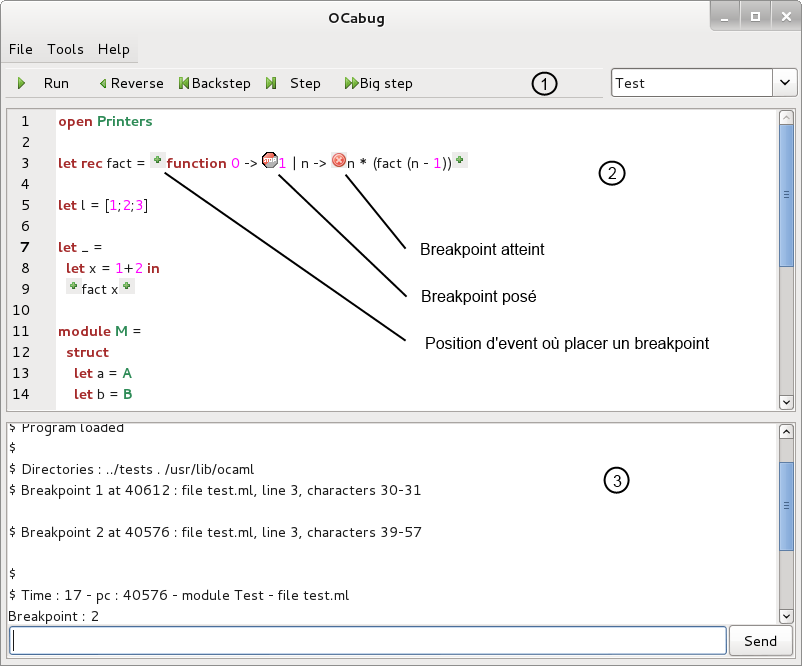
\includegraphics{screen_exec}

\begin{enumerate}
\item Barre d'outils et séléction du module à afficher
\item Affichage du fichier source du module courrant enrichi des événements de débogage activable
\item Informations textuelles et invite de commande
\end{enumerate}

L'utilisateur a activé deux ``breakpoints'' en cliquant sur les ``+'' présent dans l'affichage du source.
Il démarre ensuite le programme en appuyant sur \emph{Run} qui s'arrête au premier breakpoint rencontré,
changeant temporairement son icône ``Stop'' par un ``X'' rouge.

\subsection{Barre d'outils}

Les différents boutons incluent dans la barre d'outils réunissent les commandes les plus communes lors de l'utilisation:
\begin{itemize}
\item Run -- Permet de lancer le programme. Celui-ci s'arrêtera lorsqu'un breakpoint sera rencontré ou simplement à la fin du programme.
\item Reverse -- Action symétrique au Run; Parcours le programme en sens inverse toujours en s'arrêtant au breakpoint ou au début du programme.
\item Backstep -- Recule d'un événement de débogage.
\item Step -- Avance d'un événement de débogage
\item Big step -- Avance au prochain événement en omettant ceux de module différent.
\item Liste des modules -- Permet de basculer l'affichage des différents fichiers sources présents.
\end{itemize}

\subsection{Code source}

Le panneau affichant le code source a plusieurs emplois. Premièrement, la visualisation
du code source des différents modules du programme. Il permet également de poser des
breakpoints dans le code au niveau des événements du débogage.

% todo : code visuels des icones

\subsection{Toplevel}


%transition toplevel -> ocamldebug
\section{Placement par rapport à Ocamldebug}
%les fonctionnalités originelles sont intactes => toplevel
%organisation du code - couche d'ocamldebug
%nécessite le compilo + lablgtk
\section{Implémentation des extensions}
\section{Améliorations possibles}


\chapter{Annexes}

\section{Exemples}

\end{document}
